\documentclass[a4paper,10pt]{article}
%\documentclass[a4paper,10pt]{scrartcl}

\usepackage{../mystyle}

\setromanfont[Mapping=tex-text]{Linux Libertine O}
% \setsansfont[Mapping=tex-text]{DejaVu Sans}
% \setmonofont[Mapping=tex-text]{DejaVu Sans Mono}

\title{\sc Einführung in die Komplexe Analysis \\ \Large Blatt 1}
\author{Jendrik Stelzner}
\date{\today}

\begin{document}
\maketitle





\section{(Real und Imaginärteile)}
Es ist
\[
 \frac{i+1}{i-1} = \frac{i+1}{i(1+i)} = \frac{1}{i} = -i,
\]
und
\[
 \frac{3+4i}{2-i} = \frac{(3+4i)(2+i)}{(2-i)(2+i)} = \frac{2+11i}{5} = \frac{2}{5} + \frac{11}{5}i.
\]
Da $i^2 = -1$ (also insbesondere $i^4 = 1$) ist für alle $n \in \Z$
\[
 i^n =
 i^{(n \bmod 4)}
 \begin{cases}
   1 & \text{ falls } n \equiv 0 \mod 4, \\
   i & \text{ falls } n \equiv 1 \mod 4, \\
  -1 & \text{ falls } n \equiv 2 \mod 4, \\
  -i & \text{ falls } n \equiv 3 \mod 4.
 \end{cases}
\]
Schließlich ist
\[
 \left(\frac{1-i\sqrt{5}}{3}\right)^n
 = \Re \left( \left(\frac{1-i\sqrt{5}}{3}\right)^n \right) + i \Im \left( \left(\frac{1-i\sqrt{5}}{3}\right)^n \right)
\]
und
\begin{align*}
 \sum_{k=1}^7 \left(\frac{1+i}{\sqrt{2}}\right)^k
 &= \sum_{k=1}^7 e^{ik\pi/4}
 = \sum_{k=1}^3 e^{ik\pi/4} + \sum_{k=4}^7 e^{ik\pi/4} \\
 &= \sum_{k=1}^3 e^{ik\pi/4} + \sum_{k=0}^3 e^{ik\pi/4+i\pi} \\
 &= -1 + \sum_{k=1}^3 e^{ik\pi/4} + \sum_{k=1}^3 -e^{ik\pi/4} \\
 &= -1.
\end{align*}
Die entsprechenden Real- und Imaginärteile ergeben sich durch direktes Ablesen.





\section{(Betrag und Argument)}
Es ist
\[
 |1+3i| = \sqrt{1+3^2} = \sqrt{10} \text{ und } \arg (1+3i) = \arctan 3.
\]
Wegen der $2\pi$-Periodizität der Funktion $\R \to \C, t \mapsto e^{it}$ ist
\begin{align*}
 z_1
 &= (1+i)^9 - (1-i)^9
 = \left(\sqrt{2}e^{i\pi/4}\right)^9 - \left(\sqrt{2}e^{-i\pi/4}\right)^9 \\
 &= 2^{9/2} (e^{i\pi/4}-e^{i\pi/4})
 = 16 ((1+i)-(1-i)) \\
 &= 32i,
\end{align*}
also
\[
 |z_1| = 32 \text{ und } \arg z_1 = \frac{\pi}{2}.
\]
Da $i^2 = -1$ und $i^4 = 1$ ist $ z_2 = i^{2014} = -1$, also
\[
 |z_2| = 1 \text{ und } \arg z_2 = \pi.
\]
Für $a \in \R$ und $z_3 = \frac{1+ia}{1-ia}$ ist
\[
 \left|z_3\right|
 = \frac{|1+ia|}{|1-ia|}
 = \frac{|1+ia|}{\left|\overline{1+ia}\right|}
 = 1,
\]
und da
\[
 \arg (1+ia) = \arctan a \text{ und } \arg (1-ia) = \arctan -a = - \arctan a.
\]
ist
\[
 \arg z_3 = \arg (1+ia) - \arg (1-ia) = 2 \arctan a.
\]
Für alle $n \in \Z$ und
\[
 z_n = (i-1)^n = \left(\sqrt{2}e^{i3\pi/4}\right)^n = 2^{n/2} e^{in3\pi/4}
\]
ist $|z_n| = 2^{n/2}$ und $n\frac{3}{4}\pi$ ein Argument von $z_n$.





\section{(Bestimmte Teilmengen)}


\subsection{}
Da $\Im(z) = 0 \Leftrightarrow z \in \R$ für alle $z \in \C$, und für alle $t \in \R, z \in \C$
\[
 \frac{z-3}{1+i} = t \Leftrightarrow z = 3+t(1+i)
\]
ist
\begin{align*}
 A_0
 &= \left\{ z \in \C : \Im\left( \frac{z-3}{1+i} \right) = 0 \right\}
 = \left\{ z \in \C : \frac{z-3}{1+i} \in \R \right\} \\
 &= \{ 3+t(1+i) : t \in \R \}.
\end{align*}
Es handelt sich bei $A_0$ also um eine Gerade.

Analog ergibt sich nun auch, dass
\begin{align*}
 A_+
 &= \left\{z \in \C : \Im\left( \frac{z-3}{1+i} \right) > 0 \right\} \\
 &= \left\{3 + t(1+i) + y(i-1) : t \in \R, y \in \R^+\right\}
\end{align*}
und
\begin{align*}
 A_-
 &= \left\{z \in \C : \Im\left( \frac{z-3}{1+i} \right) > 0 \right\} \\
 &= \left\{3 + t(1+i) + y(i-1) : t \in \R, y \in \R^-\right\}.
\end{align*}
Es ist also $A_+$ der Teil der komplexen Ebene, der über $A_0$ liegt, und $A_-$ der Teil der komplexen Ebene, der unter $A_0$ liegt.
Zusammengefasst ergibt sich die folgende Skizze.

\begin{center}
 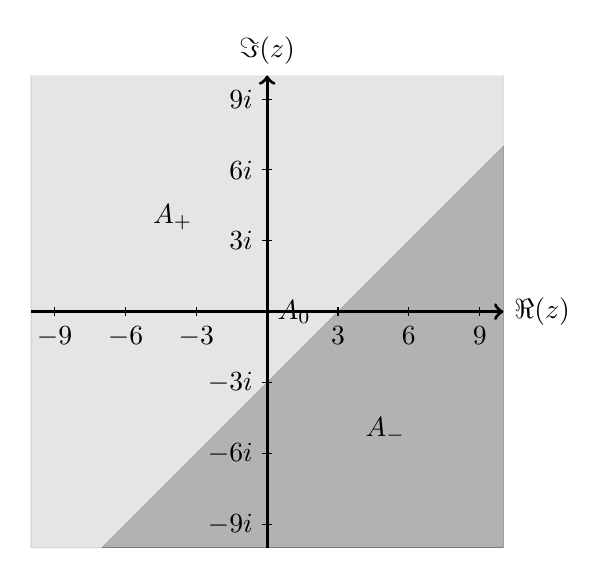
\begin{tikzpicture}[scale=0.3,domain=-7:10]
  \draw[very thick,->] (-10,0) -- (10,0) node[anchor=west] {$\Re(z)$}; % Re-Achse
  \draw[very thick,->] (0,-10) -- (0,10) node[anchor=south] {$\Im(z)$}; % Im-Achse
  % Beschriftung der Re-Achse
  \foreach \x in {-9,-6,-3,3,6,9}
   \draw (\x,1/5) -- (\x,-1/5) node[anchor=north] {$\x$};
  % Beschriftung der Im-Achse
  \foreach \y in {-9,-6,-3,3,6,9}
   \draw (1/5,\y) -- (-1/5,\y) node[anchor=east] {$\y i$};
  % Plote A_0
  \draw[thick] plot function {-3+x} node[anchor=west] {$A_0$};
  % Zeichne A_+ ein
  \draw[fill=black,opacity=0.1] (-10,10) -- (-10,-10) -- (-7,-10) -- (10,7) -- (10,10);
  \draw (-4,4) node {$A_+$};
  % Zeichne A_- ein
  \draw[fill=black,opacity=0.3] (-7,-10) -- (10,-10) -- (10,7);
  \draw (5,-5) node {$A_-$};
 \end{tikzpicture}
\end{center}


\subsection{}
Es ist $B = \emptyset$, denn für alle $z \in B$ ist
\[
 i = 3z\bar{z}+iz-i\bar{z}+2 = 3|z|^2 -2\Im(z) +2 \in \R.
\]
Die zeichnerische Darstellung der leeren Menge lassen wir dem geneigten Leser als kreative Übung.


\subsection{}
Es ist
\[
 C
 = \left\{z \in \C \left| \left|z-\frac{1}{\sqrt{2}}\right|^2 \left|z+\frac{1}{\sqrt{2}}\right|^2 = \frac{1}{4} \right.\right\}
 = \left\{z \in \C \left| \left|z^2-\frac{1}{2}\right| = \frac{1}{2} \right.\right\}.
\]
Es ist also $C$ das Urbild des Kreises mit Radius $1/2$ um den Mittelpunkt $1/2$ unter der Abbildung $z \mapsto z^2$.

Um dieses Urbild zu skizzieren betrachten wir daher zunächst das Urbild eines einzelnen Punktes $z = r e^{i\varphi}$, $r \geq 0$, welcher im oberen Qudranten der komplexen Ebene liegt (d.h. $\Im(z), \Re(z) \geq 0$). Da dieses gerade aus den beiden Punkten $\sqrt{r} e^{i\varphi/2}$ und $-\sqrt{r}e^{i\varphi/2}$ besteht, ergibt sich für den gesamten Kreis das Urbild wie in der Abbildung.

\begin{figure}[!ht]\centering
  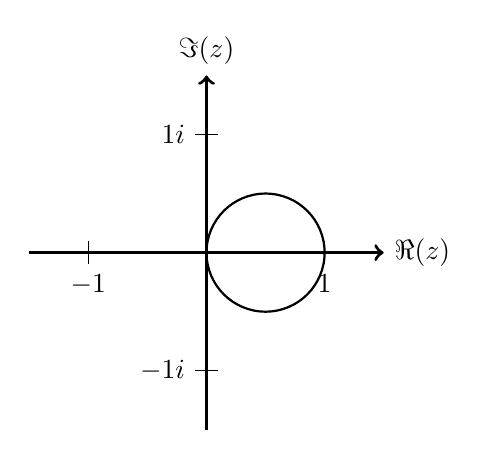
\begin{tikzpicture}[scale=1.5]
  \draw[very thick,->] (-1.5,0) -- (1.5,0) node[anchor=west] {$\Re(z)$}; % Re-Achse
  \draw[very thick,->] (0,-1.5) -- (0,1.5) node[anchor=south] {$\Im(z)$}; % Im-Achse
  % Beschriftung der Re-Achse
  \foreach \x in {-1,1}
   \draw (\x,1/10) -- (\x,-1/10) node[anchor=north] {$\x$};
  % Beschriftung der Im-Achse
  \foreach \y in {1,-1}
   \draw (1/10,\y) -- (-1/10,\y) node[anchor=east] {$\y i$};
  % Der Kreis
  \draw[thick] (1/2,0) circle (1/2);;
 \end{tikzpicture}
 \begin{tikzpicture}[scale=1.5]
  \draw[very thick,->] (-1.5,0) -- (1.5,0) node[anchor=west] {$\Re(z)$}; % Re-Achse
  \draw[very thick,->] (0,-1.5) -- (0,1.5) node[anchor=south] {$\Im(z)$}; % Im-Achse
  % Beschriftung der Re-Achse
  \foreach \x in {-1,1}
   \draw (\x,1/10) -- (\x,-1/10) node[anchor=north] {$\x$};
  % Beschriftung der Im-Achse
  \foreach \y in {1,-1}
   \draw (1/10,\y) -- (-1/10,\y) node[anchor=east] {$\y i$};
  % Das Urbild
  % In Polarkoordinaten: sqrt(sin(t/2)) e^{i(π-t)/4} für 0 <= t <= π
  \tkzInit[xmin=-1,xmax=1,xstep=1,ymin=-1,ymax=1,ystep=1]
  \tkzFctPar[thick,samples=400,domain=0:2*pi]{sqrt(sin(t/2))*cos((pi-t)/4)}{sqrt(sin(t/2))*sin((pi-t)/4)}
  \tkzFctPar[thick,samples=400,domain=0:2*pi]{-sqrt(sin(t/2))*cos((pi-t)/4)}{sqrt(sin(t/2))*sin((pi-t)/4)}
 \end{tikzpicture}
 \caption{Der Kreis (links) und sein Urbild (rechts).}
\end{figure}
(Man beachte etwa, dass die imaginäre Achse als Tangente des Kreises der Winkelhalbierende, bzw. deren konjugiertes, als Tangente von $C$ entspricht.)






\section{(Kleine Stereograpische Projektion)}
Wir bemerken zunächst, dass der Ausdruck $(i\lambda+1)/(i\lambda-1)$ für alle $\lambda \in \R$ wohldefiniert ist, da stets $i\lambda-1 \neq 0$. Für alle $\lambda \in \R$ ist auch $i\lambda+1 \neq i\lambda-1$ (da $1 \neq -1$) und daher $(i\lambda+1)/(i\lambda-1) \neq 1$. Schließlich ist für alle $\lambda \in \R$
\[
 \left| \frac{i\lambda+1}{i\lambda-1} \right|
 = \frac{|i\lambda+1|}{|i\lambda-1|}
 = \frac{\sqrt{\lambda^2+1}}{\sqrt{\lambda^2+1}}
 = 1.
\]
Die Abbildung
\[
 \psi : \R \to S^1 \setminus \{1\}, \lambda \mapsto \frac{i\lambda+1}{i\lambda-1}
\]
ist also wohldefiniert.

Da jedes $z \in S^1 \setminus \{1\}$ eine eindeutige Darstellung als $z = e^{i\varphi}$ mit $\varphi \in (0,2\pi)$ hat, genügt es zum Nachweis der Bijektivität von $\psi$ zu zeigen, dass es für alle $\varphi \in (0,2\pi)$ genau ein $\lambda \in \R$ gibt, so dass $\varphi$ ein Argument von $\psi(\lambda)$ ist.

Hierfür bemerken wir für $\lambda \in \R$, dass $\arctan \lambda$ ein Argument von $i \lambda + 1$ ist und $-\pi - \arctan \lambda$ ein Argument von $i \lambda - 1$.

Für alle $\lambda \in \R$ ist daher
\[
 \arctan \lambda - (-\pi - \arctan \lambda)
 = \pi + 2\arctan \lambda
\]
ein Argument von $\psi(\lambda)$. Da $\arctan : \R \to (-\pi/2,\pi/2)$ bijektiv ist zeigt dies nach der obigen Überlegung die Bijektivität von $\psi$.





\section{(Verschärfte Dreiecksungleichung)}
Seien $z, w \in \C$ zunächst beliebig aber fest, wobei $z = x+iy$ und $w = u+iv$ mit $x,y,u,v \in \R$. Wir zeigen zunächst, dass $|z+w| \leq |z|+|w|$. Da $|z+w|, |z|+|w| \geq 0$ ist
\begin{align*}
                &\, |z+w| \leq |z|+|w| \\
 \Leftrightarrow&\, |z+w|^2 \leq (|z|+|w|)^2 \\
 \Leftrightarrow&\, (x+u)^2 + (y+v)^2 \leq (x^2+y^2) + 2|zw| + (u^2+v^2) \\
 \Leftrightarrow&\, xu+yv \leq |zw|. \tag{1} \label{eqn: Fallunterscheidung}
\end{align*}
Ist $xu+yv < 0 \leq |zw|$ so zeigt dies die Ungleichung. Ist hingegen $xu+yv \geq 0$ so ergibt sich durch weiteres Umformen, dass
\begin{align*}
                &\, xu + yv \leq |zw| \\
 \Leftrightarrow&\, (xu+yv)^2 \leq |zw|^2 = |z|^2 |w|^2 = (x^2+y^2)(u^2+v^2) \\
 \Leftrightarrow&\, 2xuyv \leq x^2v^2 + y^2u^2 \\
 \Leftrightarrow&\, 0 \leq (xv-yu)^2, \tag{2} \label{eqn: Determinante}
\end{align*}
was offenbar gilt. Dies zeigt die gewünschte Ungleichung. (Der aufmerksame Leser merkt natürlich, dass bereits \eqref{eqn: Fallunterscheidung} aufgrund der Cauchy-Schwarz-Ungleichung erfüllt ist.)

Wir behaupten nun, dass die Gleichheit $|z+w| = |z|+|w|$ für $z, w \in \C$ genau dann gilt, wenn $z = 0$ oder $w = 0$ oder es ein $\lambda > 0$ gibt mit $w = \lambda z$. Dass die Gleichheit in diesen Fällen gilt ist klar (im letzten der drei Fälle gilt \[
 |z+w| = |(1+\lambda)z| = (1+\lambda)|z| = |z| + \lambda|z| = |z| + |\lambda z| = |z|+|w| ).
\]
Ist hingegen $|z+w| = |z|+|w|$, so ergibt sich, indem man die obige Herleitung mit Gleichheit statt der Abschätzung $\leq$ wiederholt, aus der \eqref{eqn: Determinante} entsprechenden Gleichung, dass
\[
 0 = (xv-yu)^2 \Rightarrow 0 = xv-yu = \det \vect{x&u\\y&v}.
\]
Dies zeigt, dass $(x,y), (v,u) \in \R^2$ linear abhängig sind, es also ein $\lambda \in \R$ gibt mit $(u,v) = \lambda (x,y)$. Aus der \eqref{eqn: Fallunterscheidung} entsprechenden Gleichung ergibt sich weiter, dass
\[
 0
 \leq |zw| = xu+yv
 = \vect{x\\y} \cdot \vect{u\\v}
 = \lambda \vect{x\\y} \cdot \vect{x\\y}
 = \lambda \left\|\vect{x\\y}\right\|^2,
\]
also im Falle $(x,y), (u,v) \neq 0$ (und damit insbesondere $\|(x,y)\|^2 > 0$), dass $\lambda > 0$ sein muss.

Die umgekehrte Dreiecksungleichung ergibt sich daraus, dass nach der bereits gezeigten Ungleichung für alle $z, w \in \C$
\begin{gather*}
 |z| = |w+z-w| \leq |w| + |z-w| \Rightarrow |z|-|w| \leq |z-w| \text{ und} \\
 |w| = |z+w-z| \leq |z|+|w-z| \Rightarrow |w|-|z| \leq |w-z| = |z-w|,
\end{gather*}
also
\[
 ||z|-|w|| = \max \{ |z|-|w|, |w|-|z|\} \leq |z-w|.
\]
Die auf dem Aufgabenblatt angegebene Form ergibt sich nun für alle $z, w \in \C$ durch
\[
 ||z|-|w|| =||z|-|-w|| \leq |z-(-w)| = |z+w|.
\]

Wir behaupten, dass die Gleichheit $||z|-|w|| = |z+w|$ genau dann gilt, wenn $z=0$ oder $w=0$ oder $w = -\lambda z$ für ein $\lambda > 0$. Ist $z = 0$ oder $w = 0$ so ist die Gleichheit offenbar erfüllt, und ist $w = -\lambda z$ für ein $\lambda > 0$, so ist
\begin{align*}
 |z+w|
 &= |(1-\lambda)z| = |1-\lambda| |z|
 =
 \begin{cases}
  (1-\lambda) |z| & \text{falls } \lambda \leq 1 \\
  (\lambda-1) |z| & \text{falls } \lambda > 1
 \end{cases} \\
 &=
 \begin{cases}
  |z|-|w| &\text{falls } \lambda \leq 1 \\
  |w|-|z| &\text{falls } \lambda > 1
 \end{cases}
 = \max\{|z|-|w|, |w|-|z|\} \\
 &= ||z|-|w||.
\end{align*}
Man bemerke hierfür, dass $|z| \geq \lambda |z| = |w|$ für $\lambda \leq 1$ und $|z| \leq \lambda |z| = |w|$ für $\lambda > 1$.

Ist andererseits $||z|-|w|| = |z+w|$ mit $z, w \neq 0$, so können wir o.B.d.A. davon ausgehen, dass $|z| \geq |w|$ und erhalten so, dass
\[
 |z|-|w| = |z+w| \Rightarrow |z| = |z+w|+|w| = |z+w| + |-w|.
\]
Es ist nach der obigen Diskussion für Bedingungen von Gleichheit bei der normalen Dreiecksungleichung also $z+w=0$ (also $w = -z$) oder $-w = 0$ (was wir wegen $w \neq 0$ ausschließen können) oder $z+w = - \lambda w$ und damit $w = - \frac{1}{1+\lambda} z$ für ein $\lambda > 0$.






















\end{document}
